
\documentclass[conference]{IEEEtran}
\usepackage{blindtext, graphicx, float}

\usepackage{amssymb}
\usepackage{hyperref}
\usepackage{listings}

\usepackage[utf8]{inputenc}
\usepackage[portuguese, american]{babel}
\usepackage[justification=centering]{caption}


\usepackage{biblatex}
\addbibresource{references.bib}


%% Table colores %%
\usepackage[table,xcdraw]{xcolor}

%% HEADER and FOOTER %%
\usepackage{fancyhdr}
\pagestyle{fancy}
\fancyhf{}
\rhead{\emph{University of Minho}}
\lhead{\emph{Integrated Project - July 2015}}
\rfoot{\thepage}

\begin{document}
%
% paper title
\title{Exploring parallel enumeration algorithms to improve efficiency to solve the SVP}


% author names and affiliations
% use a multiple column layout for up to three different
% affiliations
\author{\IEEEauthorblockN{Authors:\\Hélder Gonçalves\\heldergoncalves92@gmail.com\\
and João Magalhães\\jpfmm123@gmail.com}
%\IEEEauthorblockA{University of Minho}
\and
\IEEEauthorblockN{Co-Advisor:\\Artur Mariano}
\IEEEauthorblockA{Technical University of Darmstadt\\artur.mariano@sc.tu-darmstadt.de}
\and
\IEEEauthorblockN{Advisor:\\Alberto Proença}
\IEEEauthorblockA{University of Minho\\aproenca@di.uminho.pt}
}

% make the title area
\maketitle

%%%%%%%%%%%%%%%%%%%%%%%%%%%%%%%%%%%%%%%%%%
%%%%%%%%%%%%%%%%%%%%%%%%%%%%%%%%%%%%%%%%%%
%%%%%%%%%%%%%%%%%%%%%%%%%%%%%%%%%%%%%%%%%%
%%%%%%%                          %%%%%%%%%
%%%%%%%           ABSTRACT       %%%%%%%%%
%%%%%%%                          %%%%%%%%%
%%%%%%%%%%%%%%%%%%%%%%%%%%%%%%%%%%%%%%%%%%
%%%%%%%%%%%%%%%%%%%%%%%%%%%%%%%%%%%%%%%%%%
%%%%%%%%%%%%%%%%%%%%%%%%%%%%%%%%%%%%%%%%%%
\begin{abstract}

    Lattice-based cryptography methods is well known primitive from the asymmetric cryptographic primitives set. Although widely studied for decades they have gained new notoriety in the last years because it is believe in the field of cryptography that these methods can withstand attacks by upcoming quantum computers.
    Experimental testing of the algorithms properties may shed some light on its vulnerability. However the experimental results must be obtained  within reasonable time envelops, which implies efficient parallel implementations of the Enumeration algorithm able to tackle not only conventional architectures such as \emph{Intel X86}.
    In this paper we describe our implementation approach of the Enumeration algorithm on \emph{Pthreads}. As the results section shows we were able to obtain significant performance improvements over the said implementation.
    
\end{abstract}


%%%%%%%%%%%%%%%%%%%%%%%%%%%%%%%%%%%%%%%%%%
%%%%%%%%%%%%%%%%%%%%%%%%%%%%%%%%%%%%%%%%%%
%%%%%%%%%%%%%%%%%%%%%%%%%%%%%%%%%%%%%%%%%%
%%%%%%%                          %%%%%%%%%
%%%%%%%          KEYWORDS        %%%%%%%%%
%%%%%%%                          %%%%%%%%%
%%%%%%%%%%%%%%%%%%%%%%%%%%%%%%%%%%%%%%%%%%
%%%%%%%%%%%%%%%%%%%%%%%%%%%%%%%%%%%%%%%%%%
%%%%%%%%%%%%%%%%%%%%%%%%%%%%%%%%%%%%%%%%%%
\begin{IEEEkeywords}
Lattice, SVP, Enumeration, Parallelization, Pthreads.
\end{IEEEkeywords}


% For peerreview papers, this IEEEtran command inserts a page break and
% creates the second title. It will be ignored for other modes.
\IEEEpeerreviewmaketitle


%%%%%%%%%%%%%%%%%%%%%%%%%%%%%%%%%%%%%%%%%%
%%%%%%%%%%%%%%%%%%%%%%%%%%%%%%%%%%%%%%%%%%
%%%%%%%%%%%%%%%%%%%%%%%%%%%%%%%%%%%%%%%%%%
%%%%%%%                          %%%%%%%%%
%%%%%%%        Intruduction      %%%%%%%%%
%%%%%%%                          %%%%%%%%%
%%%%%%%%%%%%%%%%%%%%%%%%%%%%%%%%%%%%%%%%%%
%%%%%%%%%%%%%%%%%%%%%%%%%%%%%%%%%%%%%%%%%%
%%%%%%%%%%%%%%%%%%%%%%%%%%%%%%%%%%%%%%%%%%
\section{Introduction}
    A lattice in $R^n$ is a discrete subgroup of $R^n$ which span a real vector space $R^n$. Every lattice in $R^n$ can be generated from a basis for the vector space by forming all linear combinations with integer coefficients. A lattice may be viewed as a regular tiling of a space by a primitive cell. 

	Lattices can be applied in many contexts but it has gained importance in cryptography due to advent of quantum computing. The known public key cryptography is easily attacked by this new generation of computers. In contrast, the lattice-based cryptography is believed to be resistant to attacks from quantum computers. In cryptography NP-hard algorithms are especially attractive due to their exponential time complexity. New cryptographic approaches can be reduced to the shortest vector problem (SVP) which is known to be NP-hard making it a prime candidate to develop said approaches. 
	
    A given basis $\Lambda$ constituted by a set of totally independent linear vectors. Although a lattice can be an unbounded set  of vectors, in this paper we only consider square basis, i. e. the set size is bound by the number of basis vector such that each vector corresponds to a dimension.

    In order to increase the development performance, ensure reliability and fulfill time constrains we resort to the external library NTL. NTL encapsulates decades of performance tuning by others and provides reliability assurances that could only by achieved at the expense of large amounts of development time.
    
    The first step requires the computation of Gram–Schmidt coefficients which then will be used by the Enumeration algorithm. In order to improve the sequential implementation of the Enumeration algorithm we used a two step approach:    
    
    \emph{i)} optimization of the sequential code and its data structures\\
    \indent \emph{ii)}perform a guided parallel based on the results obtain on the previously state
    
    
    As the results actual chooses the two step described in this paper allowed us to achieved linear and/or even super-linear speedups in some cases.
  
 
%%%%%%%%%%%%%%%%%%%%%%%%%%%%%%%%%%%%%%%%%%
%%%%%%%%%%%%%%%%%%%%%%%%%%%%%%%%%%%%%%%%%%
%%%%%%%%%%%%%%%%%%%%%%%%%%%%%%%%%%%%%%%%%%
%%%%%%%                          %%%%%%%%%
%%%%%%%         Strategy         %%%%%%%%%
%%%%%%%                          %%%%%%%%%
%%%%%%%%%%%%%%%%%%%%%%%%%%%%%%%%%%%%%%%%%%
%%%%%%%%%%%%%%%%%%%%%%%%%%%%%%%%%%%%%%%%%%
%%%%%%%%%%%%%%%%%%%%%%%%%%%%%%%%%%%%%%%%%%
\section{Strategy}
 
 
 
%%%%%%%%%%%%%%%%%%%%%%%%%%%%%%%%%%%%%%%%%%
%%%%%%%%%%%%%%%%%%%%%%%%%%%%%%%%%%%%%%%%%%
%%%%%%%%%%%%%%%%%%%%%%%%%%%%%%%%%%%%%%%%%%
%%%%%%%                          %%%%%%%%%
%%%%%%%       Data Storage       %%%%%%%%%
%%%%%%%                          %%%%%%%%%
%%%%%%%%%%%%%%%%%%%%%%%%%%%%%%%%%%%%%%%%%%
%%%%%%%%%%%%%%%%%%%%%%%%%%%%%%%%%%%%%%%%%%
%%%%%%%%%%%%%%%%%%%%%%%%%%%%%%%%%%%%%%%%%%
\subsection{Data storage}
    
    Due to the huge size of the data input, it would be expensive to store it in memory thus to avoid the problem we store only the reduced basis which is computed by the Lenstra-Lenstra-Lovász (LLL) algorithm from the NTL library.
    
    The NTL is a high-performance, portable C++ library providing data structures and algorithms for manipulating signed, arbitrary length integers, and for vectors, matrices, and polynomials over the integers and over finite fields.


%%%%%%%%%%%%%%%%%%%%%%%%%%%%%%%%%%%%%%%%%%
%%%%%%%%%%%%%%%%%%%%%%%%%%%%%%%%%%%%%%%%%%
%%%%%%%%%%%%%%%%%%%%%%%%%%%%%%%%%%%%%%%%%%
%%%%%%%                          %%%%%%%%%
%%%%%%%       Pre-processing     %%%%%%%%%
%%%%%%%                          %%%%%%%%%
%%%%%%%%%%%%%%%%%%%%%%%%%%%%%%%%%%%%%%%%%%
%%%%%%%%%%%%%%%%%%%%%%%%%%%%%%%%%%%%%%%%%%
%%%%%%%%%%%%%%%%%%%%%%%%%%%%%%%%%%%%%%%%%%
\subsection{Pre-Processing stage}

    The enumeration algorithm requires the orthonormalization of the reduced basis, which is achieved through a Gram-Shmidt method.

    It is a method for orthonormalising a set of vectors in an inner product space, most commonly the Euclidean space $R^n$. The Gram–Schmidt process takes a finite, linearly independent set $S = {v1, ..., vk}$ for $k \leqslant n$ and generates an orthogonal set $S^\prime = {u1, ..., uk}$ that spans the same k-dimensional subspace of $R^n$ as $S$, i.e. as prime is the set of orthogonal basis vectors of the inner product space of $S$.
    
    The $S$ prime set is stored as a triangular matrix $\mu$ and a vector containing the squared norms although this routine is a prime candidate for vectorization, since it is only executed once with a small time footprint over the entire overall execution time such an approach yields little benefit.


%%%%%%%%%%%%%%%%%%%%%%%%%%%%%%%%%%%%%%%%%%
%%%%%%%%%%%%%%%%%%%%%%%%%%%%%%%%%%%%%%%%%%
%%%%%%%%%%%%%%%%%%%%%%%%%%%%%%%%%%%%%%%%%%
%%%%%%%                          %%%%%%%%%
%%%%%%%        Enumeration       %%%%%%%%%
%%%%%%%                          %%%%%%%%%
%%%%%%%%%%%%%%%%%%%%%%%%%%%%%%%%%%%%%%%%%%
%%%%%%%%%%%%%%%%%%%%%%%%%%%%%%%%%%%%%%%%%%
%%%%%%%%%%%%%%%%%%%%%%%%%%%%%%%%%%%%%%%%%%
\subsection{Enumeration}
    The lattice can be seen like a hypersphere. In such a scenario the enumeration process consists of enumerating the lattice inner points while progressively decreasing the hypersphere radius as the points are enumerated.
    From another perspective this model can be seen as a tree transversal, which is easier to visualize and allows easier identification of parallelization opportunities.

\begin{figure}[ht!]
\centering
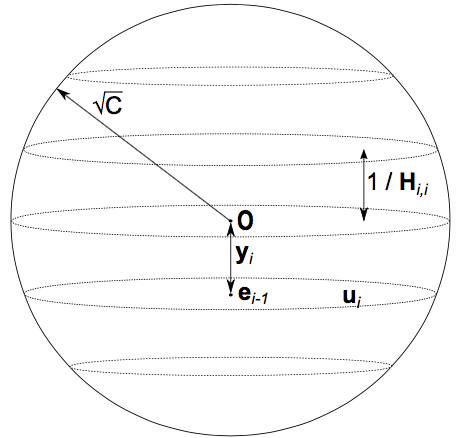
\includegraphics[width=60mm]{imgSequential/hypersphere.png}
\caption{Hypersphere representation and its sub-layers}
\end{figure}

    In Figure 1, $\sqrt C$ is the norm of the shortest vector found so far, representing its radius. The hypersphere can be sub-divided in layers of lower dimensions where the instant layer is denominated by $i$. Layer $i$ is divided in more sub-divided layers in the dimension $i-1$. 
    
    The algorithm searches a solution in all layers by starting to walk the tree at layer $n$ and finishing when revisits that layer. Walking the tree implies two methods \emph{moveUp} and \emph{moveDown}.

\begin{itemize}
\item \textbf{MoveDown} - Visits the layer with a lower dimension.
\item \textbf{MoveUP} - Visits the layer with a higher dimension.
\end{itemize}

If at any moment the algorithm reaches dimension 0, then a smaller vector exists. In such case the current smallest vector is replaced by the newly formed.

\subsection{Pseudo-Code}
To easily understand how the sequential version of the Enumeration algorithm works, we have a draft of our implementation in pseudo-code, based on Schnorr's work \cite{schnorr}.


\begin{lstlisting}[frame=single,language=C]
//Start by Initializing all the variables

while( t <= End_Dimension ){
    //Compute cT[i]
    if( cT[t] < current_Norm ){
        if( t > 0 )
            moveDown();
        else
            updateVector();
    }else
        moveUp();
}
\end{lstlisting}

\subsection{Profiling}
In order to identify hotpots in the code we used gprof. Table I shows the profiler results, namely the number of calls and the percentage of overall time for each of the code functions.
The profiling took 404.70 seconds longer.

\begin{table}[ht!]
\centering
\label{my-label}

\begin{tabular}{|c|c|c|}
\hline
\rowcolor[HTML]{C0C0C0} 
{\color[HTML]{000000} Function} & {\color[HTML]{000000} Time (\%)} & {\color[HTML]{000000} Nº of Calls} \\ \hline
ENUM                            & 98,5                             & 1                                  \\ \hline
moveDown                        & 67,6                             & 3159878635                         \\ \hline
moveUp                          & 10                               & 3159878580                         \\ \hline
updateVector                    & 0,7                              & -                                  \\ \hline
\end{tabular}
\caption{GPROF profiling results for a basis dimension of 55 and $-O3$ optimization}
\end{table}

From table \emph{I} it is trivial to conclude that \emph{moveUp} and \emph{moveDown} have an extremely high number pf function calls and most importantly \emph{moveDown} accounts for the majority of the execution time.

\section{Sequential enumeration algorithm optimization}
After a careful examination of the \emph{C} code and the compiler generated \emph{Assembly} code several hotspots were identified. 

\subsubsection{Power Decomposition}
The first one was the decomposition of the power function. The power function is a very heavy function and must be avoid when the exponent is always the same, and that was the case $(a + b)^2$. So, to do the decomposition we applied some math rules.
\begin{equation}
(a + b)^2 = a^2 + 2ab + b^2
\end{equation}

\begin{equation}
(a + b)^2 = (a + b) \times (a + b)
\end{equation}

To solve this problem there are two possible solutions. The first one is slower than the second one. This happens because to compute the first solution it is necessary to compute at least 4 multiply operations and 2 sum operations. In contrast, to compute the second option just is necessary compute 1 sum operation and a multiply operation. This is possible because is done the sum to a local variable and then the value multiply itself. 

\subsubsection{Avoid Computation}
A careful examination of the usage of $cT[t]$ revealed we could postpone its computation to the moment exactly prior to its use. 

\subsubsection{Inline}
As gprof reported, the functions \emph{moveUp} and \emph{moveDown} are constantly called which implies all the necessary operations such as stack creation, returning, ... To avoid function call overhead, both funcions were inlined which not only removes the call overhead but also increases the compiler opportunities for automatic optimization.

    Now to try to increase the performance of the current algorithm, were tried greater depth implementations.
    
\subsubsection{Memoizing}
In most cases performance improvement has a careful balancing between computations cost and memory access latency. In this particular application we exploited a memoization technique for $y[t]$ and empirically determined that it was not worth while paying the cost of memory access.

    Although it seems a good practice, it got worst results because this computation is small enough to not provide a best result. That happens because computing it is faster than getting it from the memory.
    
\subsubsection{Map-Reduce}
Map-Reduce is a technique in which we map the problem into different sub problems and then reduce it all to have the final result.
In function \emph{moveDown} we saw an opportunity to vectorize a \emph{for} cycle, taking advantages of the possibility of computing various values at the same time.
In this case we had a problem because in every cycle iteration we would store the value in the same memory location.
We tried to apply the Map-Reduce concept in this case by creating an array of values, dividing the iterations between those values and then sum all the values of that array, which meant we could vectorize the first cycle.
Unfortunately, the last dependency was very hard to turn around. Although the increase achieved on vectorization was a great advantage, it is lost on the second cycle when the sum was done.
    
\subsection{Improvement Results}
    Table III show us the results of tests made for a 55 basis dimension. After all the tests, the \emph{Inline} version has the best speed up. Despite attempts to advanced improvements, we could not achieve better results than the \emph{Inline}, for the reasons explained above.
    
\begin{table}[ht!]
\centering
\label{my-label}

\begin{tabular}{|c|c|c|}
\hline
\rowcolor[HTML]{C0C0C0} 
{\color[HTML]{000000} Test Version} & {\color[HTML]{000000} Time (seconds)} & {\color[HTML]{000000} SpeedUp} \\ \hline
Source                          & 407,70            & 1,00          \\ \hline
Inline                          & 225,23            & 1,80          \\ \hline
Save \& Re-use                  & 274,54            & 1,47          \\ \hline
Map-Reduce                      & 240,09            & 1,69          \\ \hline
\end{tabular}
\caption{Improvements tests results}
\end{table}
    
\subsection{Cache misses}
The average cache misses are an important measure of application performance. Figure 2 shows the percentage of instruction and data misses for dimension 55. 

\begin{figure}[ht!]
\centering
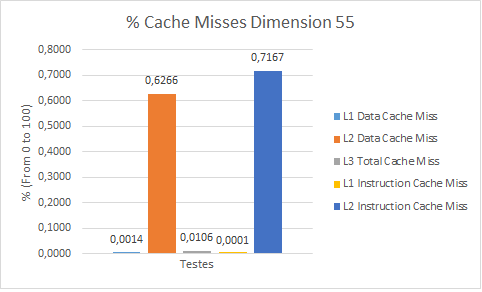
\includegraphics[width=75mm]{imgSequential/Cachemisses}
\caption{Cache miss percentage for the inline version, dimension 55}
\end{figure}

The total values can be see in table III. 

\begin{table}[H]
\centering
\label{my-label}

\begin{tabular}{|c|c|}
\hline
\rowcolor[HTML]{C0C0c0} 
{\color[HTML]{000000} Counter} & {\color[HTML]{000000} Value}  \\ \hline
PAPI\_LD\_INS                     & 369695637512                 \\ \hline
PAPI\_ST\_INS                     & 614658154544                 \\ \hline
Total instructions                & 984353792056                 \\ \hline
PAPI\_L1\_DCM                     & 13648217                     \\ \hline
PAPI\_L2\_DCM                     & 85526                        \\ \hline
PAPI\_L3\_TCA                     & 131845                       \\ \hline
PAPI\_L3\_TCM                     & 14                           \\ \hline
PAPI\_L1\_ICM                     & 469907                       \\ \hline
PAPI\_L2\_ICM                     & 3368                         \\ \hline
PAPI\_FP\_OPS                     & 224287468034                 \\ \hline
Time(s)                           & 199                          \\ \hline
FLOPS                             & 1127072704                   \\ \hline
Operational Intensity             & 1257893,643                  \\ \hline
\end{tabular}
\caption{Cache miss values for the inline version, dimension 55}
\end{table}
    
As we can see in Figure 2, we have a very low percentage of cache misses, with the maximum value being 0.72\% for the L2 instruction cache miss. The operational intensity is measured by the number of floating point operations per second divided by the number of bytes that was transferred by the memory. In this case we have more than 200 billion floating point operations and 199 seconds, so we have about 1 billion floating operations per second. Since we only have 14 times 64 bytes transferred from memory, we have an operational intensity of more than 1 million. This definitely means that we have a compute bound problem. 
Since we have a compute bound problem, we do not need to restructure the data to make it more memory friendly.

%%%%%%%%%%%%%%%%%%%%%%%%%%%%%%%%%%%%%%%%%%
%%%%%%%%%%%%%%%%%%%%%%%%%%%%%%%%%%%%%%%%%%
%%%%%%%%%%%%%%%%%%%%%%%%%%%%%%%%%%%%%%%%%%
%%%%%%%                          %%%%%%%%%
%%%%%%%     Parallelization      %%%%%%%%%
%%%%%%%                          %%%%%%%%%
%%%%%%%%%%%%%%%%%%%%%%%%%%%%%%%%%%%%%%%%%%
%%%%%%%%%%%%%%%%%%%%%%%%%%%%%%%%%%%%%%%%%%
%%%%%%%%%%%%%%%%%%%%%%%%%%%%%%%%%%%%%%%%%%
\section{Paralellization}
The paralellization of the enumeration algorithm is very important, since it is possible to obtain linear, or even super linear speedups up to 20 threads, as can be seen in the results section. 
To parallelize the algorithm, Pthreads was used since it has lower overhead thread creation than OpenMP.

\subsection{Before paralellization - preparation of the code}
To divide the enumeration algorithm, the code must be prepared for paralellization. For that a new structure was created, called Enum. This structure contains the following two short values:

\begin{itemize}
\item bound - Responsible of telling the task in which dimension it must start and stop, not going further.
\item sibling - Used to tell the task what is its sibling (see subsection IV.C).
\end{itemize}

This structure also has an array of short values, called \emph{vec}. This array can either be null or of size \emph{VectorLength} (see subsection IV.D). The level is used to tell the task how much values the array has.
Finally, this structure also has a variable called type, that defines the behaviour of the task. The possible behaviours of the task are the following:

\begin{itemize}
\item 0 - the task behaves like the serial algorithm.
\item 1 - the task behaves like on type 0 but has a fixed bound, that can not be exceeded.
\item 2 - this type is part of the siblings division and it runs until its bound plus one (see subsection IV.C). This type only occurs when the sibling is 2.
\item 3 - this type is like type 2 but it must stop in its bound (see subsection IV.C).
\item 4 - this type is like type 2 but, instead of running until its bound plus one, the dimension that the task stops running must be calculated (see subsection IV.D). Like type 2, this type only occurs for sibling 2.
\end{itemize}

A structure to handle all the Enum structures was created. This structure (called LEnum) is a linked list of Enum structures and its accessed by the threads when they are created or when they complete a task. When a thread requests a new task, that task is removed from LEnum. If no tasks are left in the linked list, then the thread will wait until all threads end their work to end the program.


\subsection{First attempt - Blindly divide the dimensions}
The first attempt to parallelize the code, consisted of blindly divided the dimensions. Each dimension has an associated task, in which we disregard the values of bigger dimensions and apply the algorithm starting from a given dimension (type 1 division). This division is done until a special dimension is reached, defined by the variable \emph{MAX\_DEPTH} and after that all dimensions are computed as part of the same task. 
In the Figure 3, the divisions made for a lattice with dimension 50 and \emph{MAX\_DEPTH} equal to 35 can be seen:

\begin{figure}[ht!]
\centering
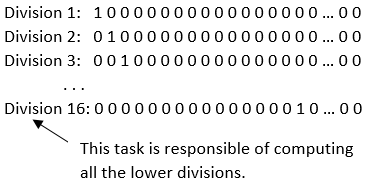
\includegraphics[width=65mm]{imgParallel/PrimeiraParalelizacao}
\caption{First parallelization division}
\end{figure}

As can be seen, there will be 16 total divisions. Each task is in charge of a given dimension and the task in charge of dimension 35 computes all the lower dimensions. It was done this way because lower dimensions have much less computation than bigger ones. 

\subsection{Second attempt - Division by siblings}
After testing the first paralellization attempt, it was discovered that the biggest dimensions would take a lot of time to compute and the code would become sequential at some point. For example, if for a lattice with 50 dimensions and even if the first task to be run was the one associated with dimension 50, it would be the last to finish making the program scale poorly.
To improve the parallelization, it was decided to divide the biggest dimensions by siblings, limited by the variable \emph{divRange}. These siblings improve the performance of the program a lot, by further dividing the previous tasks into four each. The siblings  0, 1 and -1 behave the same way (type 3), but sibling 2 behaves in a special way (type 2), in  which the bound of the task is equal to the others plus one. The way it works is really simple, imagine if we had a previous task for dimension 50. If we use siblings, we are forcing the value associated with dimension 50 to be 1, and the value for dimension 49 is set with the value of the sibling. 

\begin{figure}[ht!]
\centering
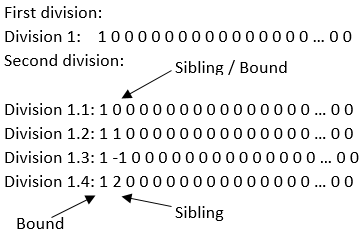
\includegraphics[width=65mm]{imgParallel/SegundaParalelizacao}
\caption{Second parallelization division}
\end{figure}

\subsection{Final parallelization}
After the second parallelized algorithm was tested, it was noticed that the tasks in charge of sibling 0 were still taking too much time to complete. To resolve this problem, further division of the tasks was obtained by creating vectors that force a given number of values (which varies with the variable \emph{VectorLength}) to be fixed. After applying this vector, siblings were use to divide the tasks even more. 
To avoid wasting time in the generation of these vectors, they are all generated once and put into a matrix. After this matrix is generated, an iteration is made from the number of dimensions until the variable \emph{CreateRange}, creating a task for each sibling of each vector of each dimension. After this creation, the matrix containing the vectors is free'd.
With the division done this way, there were much more divisions than before and the tasks were more fine-grained. A new type of behaviour similar to type 2 (in which tasks would run until the dimension defined by its bound plus one) was used to make the algorithm run all the possible combinations. In this new type (type 4) the dimension where the task stops is calculated by the number of sequential array positions that have the number 2. 

Figure 5 has a small example of vector generation for \emph{VectorLength} equal to 2:

\begin{figure}[ht!]
\centering
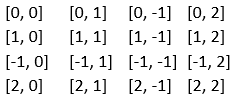
\includegraphics[width=43mm]{imgParallel/GeracaoVetores}
\caption{Vector generation}
\end{figure}

For each of these vectors, there are four divisions, corresponding with the four siblings being used, as can be seen in Figure 6, for vector [1, 2, -1]:

\begin{figure}[ht!]
\centering
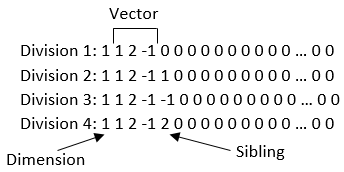
\includegraphics[width=65mm]{imgParallel/ParalelizacaoFinal}
\caption{Final parallelization}
\end{figure}

The vectors actually have one more position, which is filled with the sibling and used to compute it more easily.

The difference of behaviour for type 4 can be shown in Figure 7.

\begin{figure}[ht!]
\centering
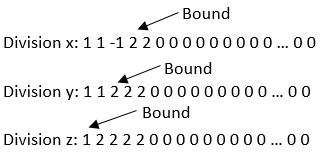
\includegraphics[width=65mm]{imgParallel/Type4}
\caption{Variation of the bound with different vectors}
\end{figure}

As can be seen, the bound of type 4 is equal to the last position of the \emph{vec} array with value 2 (from right to left), except when all the values of the array are 2, in which case the bound is equal to the dimension. 

After all types of divisions were defined, a combination of them was used to try to maximize the performance of the algorithm by improving the way the division is made. In Figure 8, the way divisions are defined and for what dimensions can be seen:

\begin{figure}[ht!]
\centering
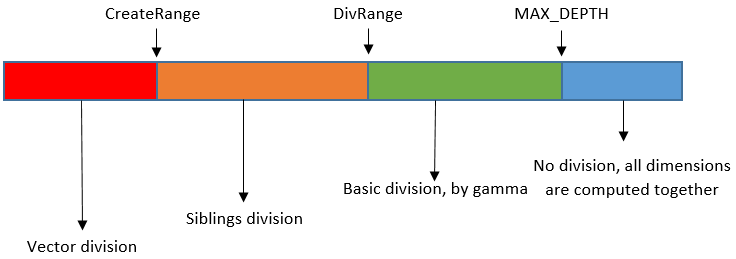
\includegraphics[width=89mm]{imgParallel/TotalDivisions}
\caption{Final divisions}
\end{figure}

\section{Results} 
\subsection{TestBed}
The algorithm was tested on nodes 652-1 and 652-2 of the search6 cluster. Every test took the entire node, so the performance would not be affected by another program or by context switches. The specification for this two nodes can be seen in Figure 8.

\begin{figure}[ht!]
\centering
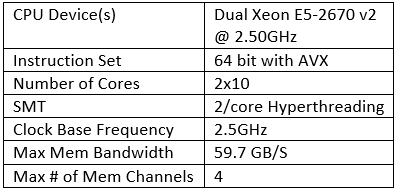
\includegraphics[width=70mm]{TestesFinais/652Specs}
\caption{Specifications for nodes 652-1 and 652-2 of the Search6 cluster}
\end{figure}


\subsection{Division variables}
For this test, the variables of the division were the following:

\begin{itemize}
\item \emph{CreateRange}: this variable was set as equal to the number of processors running the algorithm. For example, for 16 processors running for a lattice with dimension 50, then all dimensions from 50 to 35 would be divided with vectors.
\item \emph{DivRange}: set to 60\% of the lattice dimension.
\item \emph{MAX\_DEPTH}: set to 40\% of the lattice dimension.
\item \emph{VectorLengh}: In this test, a vector length of 4 (including the position of the vector reserved to the sibling) was used.
\end{itemize}

These numbers are not optimal, by far. We used them by trial and error for a specific lattice (with dimension 50) and then we applied them to all the lattices in this test. 


\subsection{Test results}


In appendix A, the results for this test can be seen. Tests were made for seeds 0 and 15 for lattices with dimensions 50, 55, 58, 60 and 65. 

With dimension 50 the speedups are constants and almost linear as it increases the number of threads what is good. On the next dimensions (55, 58 and 60) the parameters are almost perfect, especially on basis 55, having linear speedups. But are on basis 60 (seed 15) a super-linear speedup is achieved with 24 times best for 20 threads. However, the seed 0 speedup is worst. This difference between seeds is explained by the way how our implementation crosses the tree. The solution of the problem also can be on dimension 20 as can be on dimension 50. Now, if the final solution is found at the beginning of computation, the algorithm will have less sub-trees to visit than if it is found at the end, what will make it more slow.

As it was said earlier, the biggest problem of our implementation is that the numbers of divisions created are not optimal for each one of the different basis. This is clear for the speedup of base 65, specially for seed 0, that only improves for two threads as expected and after that the speedup is really bad. This happens because there are few divisions for the complexity of the computation of this dimension. A curious problem in the seed 0 was the fact of it actually takes more time to find the solution with 20 threads than it takes with 16. That happens because when it execute with 20 threads are created a bigger set of siblings with vectors and increase memory used what causes memory access issues. 

The way that the parallelization is made, the speedup really depends of the seed that is used. This is because when there is a task that is created with the vector division, first it is checked if the combination of values is possible for that lattice and only then computed if the task can provide a better solution so, if there is a seed that has a lot of tasks that do not need to be computed, augmenting the number of tasks can have a lower impact on speed than in the case where there is a need compute much more tasks.

%%%%%%%%%%%%%%%%%%%%%%%%%%%%%%%%%%%%%%%%%%
%%%%%%%%%%%%%%%%%%%%%%%%%%%%%%%%%%%%%%%%%%
%%%%%%%%%%%%%%%%%%%%%%%%%%%%%%%%%%%%%%%%%%
%%%%%%%                          %%%%%%%%%
%%%%%%%       CUDA and MIC       %%%%%%%%% 
%%%%%%%                          %%%%%%%%%
%%%%%%%%%%%%%%%%%%%%%%%%%%%%%%%%%%%%%%%%%%
%%%%%%%%%%%%%%%%%%%%%%%%%%%%%%%%%%%%%%%%%%
%%%%%%%%%%%%%%%%%%%%%%%%%%%%%%%%%%%%%%%%%%
\section{CUDA and MIC}
To help improve the performance of this algorithm, the usage of CUDA and MIC systems would probably help a lot but the code would need some major changes for that to be possible.

In the CUDA case this code lacks opportunities for vectorization, so the algorithm would have to be restructured to make the CUDA implementation possible.

In the MIC case, the implementation would be really difficult since the parallelization is implemented in Pthreads and the systems like Xeon Phi are not compatible with it. So, to implement this code in Xeon Phi the way the parallelization was made would have to chenge to OpenMP. When finally there was all the different ways to divide the work defined and tests started, there was no time to rewrite the code to OpenMP to implement it on Xeon Phi.


%%%%%%%%%%%%%%%%%%%%%%%%%%%%%%%%%%%%%%%%%%
%%%%%%%%%%%%%%%%%%%%%%%%%%%%%%%%%%%%%%%%%%
%%%%%%%%%%%%%%%%%%%%%%%%%%%%%%%%%%%%%%%%%%
%%%%%%%                          %%%%%%%%%
%%%%%%%       Future Work        %%%%%%%%%
%%%%%%%                          %%%%%%%%%
%%%%%%%%%%%%%%%%%%%%%%%%%%%%%%%%%%%%%%%%%%
%%%%%%%%%%%%%%%%%%%%%%%%%%%%%%%%%%%%%%%%%%
%%%%%%%%%%%%%%%%%%%%%%%%%%%%%%%%%%%%%%%%%%
\section{Future work}
After the work that was done in our project, there is great opportunity to further improve the performance of the algorithm. 

For example, instead of the division by vectors being made just for the number of dimensions equal to the number of threads, there must be a mathematical formula that will optimize the time the algorithm takes to run by varying the number of dimensions divided by vectors. This is true not only for variable \emph{CreateRange} but also for variables \emph{DivRange}, \emph{MAX\_DEPTH} and even \emph{VectorLength}.

Another way to further improve the algorithm is by applying a sieving optimization like extreme pruning to discard some of the branches, making the algorithm much faster. For that there was a need to resort to CUDA do compute the bounding function of the lattice and then compare the norm of each vector with the result of the bounded function instead of the current lowest vector norm.


%%%%%%%%%%%%%%%%%%%%%%%%%%%%%%%%%%%%%%%%%%
%%%%%%%%%%%%%%%%%%%%%%%%%%%%%%%%%%%%%%%%%%
%%%%%%%%%%%%%%%%%%%%%%%%%%%%%%%%%%%%%%%%%%
%%%%%%%                          %%%%%%%%%
%%%%%%%        Conclusion        %%%%%%%%%
%%%%%%%                          %%%%%%%%%
%%%%%%%%%%%%%%%%%%%%%%%%%%%%%%%%%%%%%%%%%%
%%%%%%%%%%%%%%%%%%%%%%%%%%%%%%%%%%%%%%%%%%
%%%%%%%%%%%%%%%%%%%%%%%%%%%%%%%%%%%%%%%%%%
\section{Conclusion}
In this project we managed to parallelize the enumeration algorithm in a way that linear or even super linear speedups can be achieved, specially in the case of base 60 seed 0 in which we had a speedup of 25 times for 20 threads.
In spite of this results, a lot of work can be done to further improve the algorithm, as discussed in the future work section. 

The main problem we had in this project was understanding how the code works. This took a really long time and it was only managed to do it with help of our advisors. The way the auxiliary variables had to be created / altered to enable the parallelization was something that made us loose a lot of time too, since for every new division type, the way creation and assigning of values to the auxiliary variables was made changed.

%%%%%%%%%%%%%%%%%%%%%%%%%%%%%%%%%%%%%%%%%%
%%%%%%%%%%%%%%%%%%%%%%%%%%%%%%%%%%%%%%%%%%
%%%%%%%%%%%%%%%%%%%%%%%%%%%%%%%%%%%%%%%%%%
%%%%%%%                          %%%%%%%%%
%%%%%%%      Acknowledgment      %%%%%%%%%
%%%%%%%                          %%%%%%%%%
%%%%%%%%%%%%%%%%%%%%%%%%%%%%%%%%%%%%%%%%%%
%%%%%%%%%%%%%%%%%%%%%%%%%%%%%%%%%%%%%%%%%%
%%%%%%%%%%%%%%%%%%%%%%%%%%%%%%%%%%%%%%%%%%
\section*{Acknowledgments}
We would like to thank our advisors for all the help they gave us and for always being available for all the questions we had. 
We would also like to thank Fábio Correia for all the help he gave us in understanding how the code works and what problems with the optimizaion attack first since they were the most important. 

%%%%%%%%%%%%%%%%%%%%%%%%%%%%%%%%%%%%%%%%%%
%%%%%%%%%%%%%%%%%%%%%%%%%%%%%%%%%%%%%%%%%%
%%%%%%%%%%%%%%%%%%%%%%%%%%%%%%%%%%%%%%%%%%
%%%%%%%                          %%%%%%%%%
%%%%%%%       Bibliography       %%%%%%%%%
%%%%%%%                          %%%%%%%%%
%%%%%%%%%%%%%%%%%%%%%%%%%%%%%%%%%%%%%%%%%%
%%%%%%%%%%%%%%%%%%%%%%%%%%%%%%%%%%%%%%%%%%
%%%%%%%%%%%%%%%%%%%%%%%%%%%%%%%%%%%%%%%%%%
\printbibliography
\nocite{latticeAverage}
\nocite{fabio}
\nocite{parallel}



\clearpage
\appendices
%%%%%%%%%%%%%%%%%%%%%%%%%%%%%%%%%%%%%%%%%%
%%%%%%%%%%%%%%%%%%%%%%%%%%%%%%%%%%%%%%%%%%
%%%%%%%%%%%%%%%%%%%%%%%%%%%%%%%%%%%%%%%%%%
%%%%%%%                          %%%%%%%%%
%%%%%%%       Test Results       %%%%%%%%%
%%%%%%%                          %%%%%%%%%
%%%%%%%%%%%%%%%%%%%%%%%%%%%%%%%%%%%%%%%%%%
%%%%%%%%%%%%%%%%%%%%%%%%%%%%%%%%%%%%%%%%%%
%%%%%%%%%%%%%%%%%%%%%%%%%%%%%%%%%%%%%%%%%%
\section{Test results}
Results and speedups for seeds 0 and 15 for dimensions 50, 55, 58, 60 and 65. The division variables are: \emph{CreateRange} set to dimension - number of threads; \emph{DivRange} set to 60 per cent of the dimension; \emph{MAX\_DEPTH} set to 40 per cent of the dimension and \emph{VectorLength} set to 4 (including the reserved index for the sibling).

\begin{figure}[H]
\centering
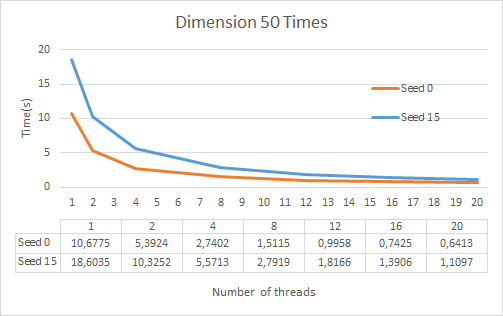
\includegraphics[width=85mm]{TestesFinais/Dimension50Times}
\caption{Dimension 50 Times}
\end{figure}

\begin{figure}[H]
\centering
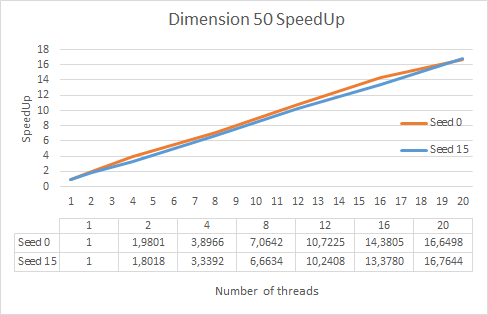
\includegraphics[width=85mm]{TestesFinais/Dimension50Speedup}
\caption{Dimension 50 Speedup}
\end{figure}

\begin{figure}[H]
\centering
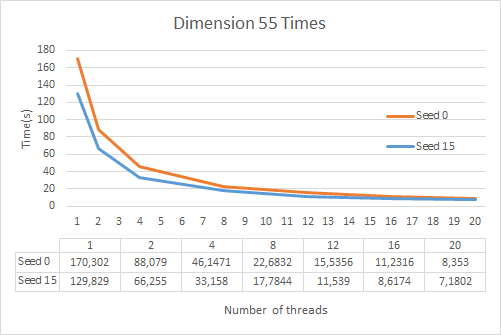
\includegraphics[width=85mm]{TestesFinais/Dimension55Times}
\caption{Dimension 55 Times}
\end{figure}

\begin{figure}[H]
\centering
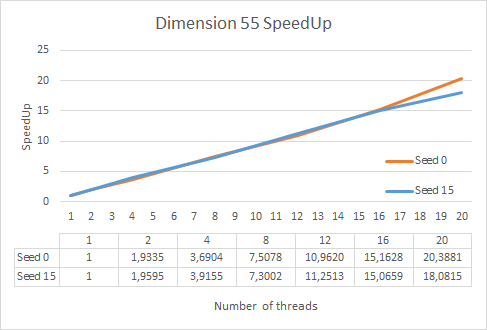
\includegraphics[width=85mm]{TestesFinais/Dimension55Speedup}
\caption{Dimension 55 Speedups}
\end{figure}

\begin{figure}[H]
\centering
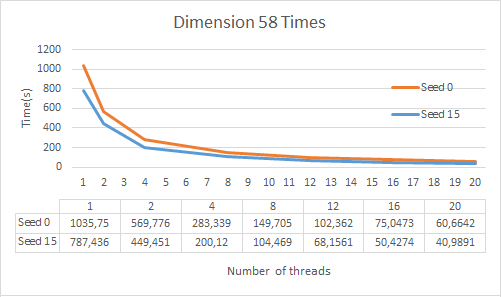
\includegraphics[width=85mm]{TestesFinais/Dimension58Times}
\caption{Dimension 58 Times}
\end{figure}

\begin{figure}[H]
\centering
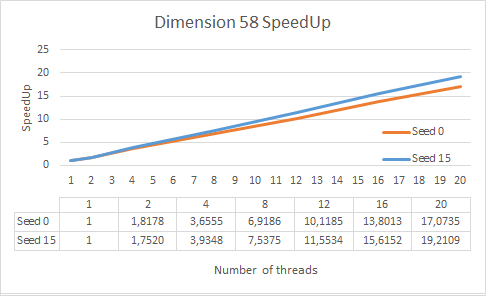
\includegraphics[width=85mm]{TestesFinais/Dimension58Speedup}
\caption{Dimension 58 Speedups}
\end{figure}

\begin{figure}[H]
\centering
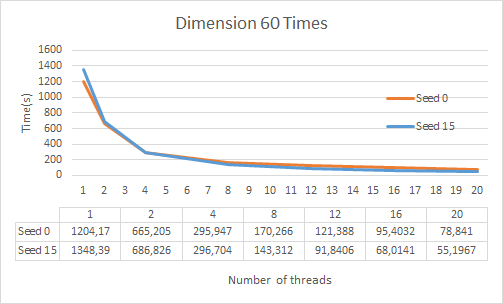
\includegraphics[width=85mm]{TestesFinais/Dimension60Times}
\caption{Dimension 60 Times}
\end{figure}

\begin{figure}[H]
\centering
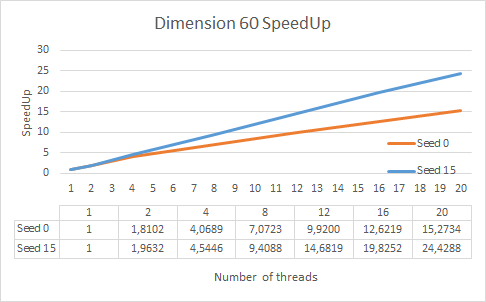
\includegraphics[width=85mm]{TestesFinais/Dimension60Speedup}
\caption{Dimension 60 Speedups}
\end{figure}

\begin{figure}[H]
\centering
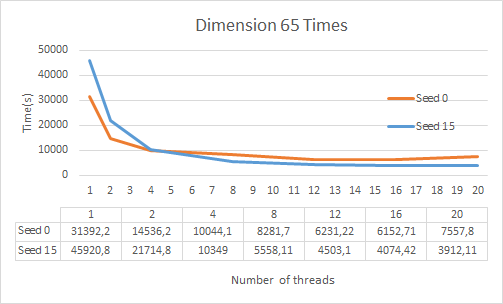
\includegraphics[width=85mm]{TestesFinais/Dimension65Times}
\caption{Dimension 65 Times}
\end{figure}

\begin{figure}[H]
\centering
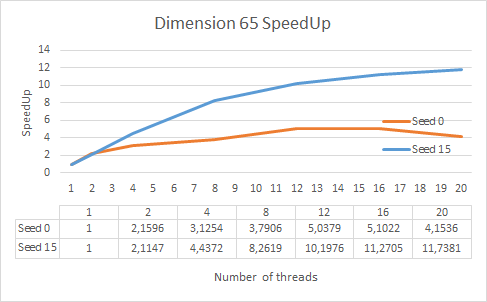
\includegraphics[width=85mm]{TestesFinais/Dimension65Speedup}
\caption{Dimension 65 Speedups}
\end{figure}

\end{document}


